% \documentclass{article}
\documentclass[twoside]{article}
\usepackage[utf8]{vietnam}
\usepackage{start/init} 
% \usepackage{microtype}
\usepackage{blindtext}
\usepackage{hyperref}
\usepackage{graphicx}
\usepackage{enumitem}
\usepackage[mathscr]{eucal}
\usepackage{amsmath, amsthm, amssymb,amsxtra,latexsym,amscd,graphics,graphpap, makeidx, tikz, color}
\usepackage{diagbox}
\usepackage{indentfirst}
\usepackage{rotating}
\usepackage{float}
\usepackage{amssymb}
\usepackage{amsmath}
\usepackage{arydshln}
\usepackage{graphicx}
\usepackage{amsbsy}
\usepackage{array}
\usepackage{epsfig}
\usepackage{natbib}
\usepackage{arydshln}

%\theorembodyfont{\slshape}
\theoremstyle{plain}
\newtheorem{definition}{Định nghĩa}[section]
\newtheorem{proposition}{Mệnh đề}[section]
\newtheorem{theorem}{Định lý}[section]
\newtheorem{lemma}{Bổ đề}[section]
\newtheorem{corollary}{Hệ quả}[section]
\newtheorem{conjecture}{Dự đoán}[section]
\newtheorem{remark}{Chú ý}[section]

\renewcommand{\thedefinition}{\arabic{section}.\arabic{definition}}
\renewcommand{\thelemma}{\arabic{section}.\arabic{lemma}}
\renewcommand{\thetheorem}{\arabic{section}.\arabic{theorem}}
\renewcommand{\thecorollary}{\arabic{section}.\arabic{corollary}}
% 
\renewcommand{\theequation}{\thesection.\arabic{equation}} % Định dạng lại số công thức
\numberwithin{equation}{section} % Đánh số công thức theo section

% Sử dụng gói caption để tùy chỉnh caption
\usepackage{caption}%* caption
% Sử dụng gói listing để hiển thị mã nguồn
\usepackage{listing}
\renewcommand*{\listlistingname}{Danh sách mã nguồn}
\DeclareCaptionLabelFormat{code_caption}{{Mã nguồn #2}}
\captionsetup[listing]{labelformat=code_caption}

% Sử dụng gói minted để đính kèm và định dạng mã nguồn
\usepackage{minted} 
\definecolor{BackgroundCode}{RGB}{242,242,235}
\setminted{
fontsize=\footnotesize, % Cỡ chữ cho mã nguồn
frame=lines, % Hiển thị đường viền xung quanh mã nguồn
framesep=2mm, % Khoảng cách giữa đường viền và nội dung mã nguồn
bgcolor=BackgroundCode, % Màu nền cho mã nguồn
% linenos, % Hiển thị số dòng ở bên trái
autogobble, % Tự động loại bỏ khoảng trắng ở đầu mỗi dòng
}
\usepackage{multirow}
\usepackage{lscape}
\usepackage{graphicx}

%%%%%%%%%%%%%%%%%%%%%%%%%%%%%%%%%%%%%%%%%%%%%%%%%%%%%%%
\begin{document}
\title{\fontsize{44pt}{0pt}\selectfont Tính toán song song}
\subtitle{\fontsize{20pt}{0pt}\selectfont Chủ đề: \break Chương trình tính tích vô hướng của 2 vector}
\author{
\textbf{Vũ Văn Nghĩa} & \textbf{20206205} \\ 
\textbf{Trần Minh Quang} & \textbf{20206209} \\ 
\textbf{Nguyễn Quốc Thái} & \textbf{20206168} \\ 
[1cm]
}
\date{\textbf{\today}}
\info{
 \textbf{Giảng viên giảng dạy: TS. Vũ Thành Nam} \\ 
 \textbf{Mã học phần: MI4364} \\ 
 \textbf{Mã lớp học: 146169} \\ 
 \textbf{Nhóm sinh viên thực hiện: Nhóm 27}
}
\usecolor{HustRed}
\logo[scale=0.6]{pictures/logotitle.png}
\maketitlepage

\tableofcontents
\newpage
\section*{Bảng đánh giá thành viên}
\phantomsection \addcontentsline{toc}{section}{Bảng đánh giá thành viên}
\begin{center}
 \begin{tabular}{|c|c|c|c|}
 \hline
 \multicolumn{3}{|c|}{\textbf{BẢNG ĐÁNH GIÁ THÀNH VIÊN}} \\ 
 \hline
 \textbf{STT} & \textbf{Họ tên} & \textbf{Nhiệm vụ} \\ \hline
 1 & Vũ Văn Nghĩa & Làm báo cáo \LaTeX \\ 
 & & Lập trình tuần tự tính tích vô hướng 2 vector \\ \hline
 2 & Trần Minh Quang & Lập trình tuần tự nhân ma trận với vector \\ 
 & & Lập trình song song nhân ma trận với vector \\ \hline
 3 & Nguyễn Quốc Thái & Lập trình song song tính tích vô hướng 2 vector \\ \hline
 \end{tabular}
\end{center}

% Danh sách 
\newpage
\listoftables
\addcontentsline{toc}{section}{Danh sách bảng}




% \newpage
\listoffigures
\addcontentsline{toc}{section}{Danh sách hình vẽ}


% \newpage
\listoflistings
\addcontentsline{toc}{section}{Danh sách mã nguồn}

\newpage
\section*{Lời mở đầu}
\phantomsection \addcontentsline{toc}{section}{Lời mở đầu}

Trong thời đại hiện nay, sự phát triển nhanh chóng của công nghệ đang thách thức với việc xử lý công việc ngày càng lớn và phức tạp. Tính toán song song là một phương pháp quan trọng để tăng cường hiệu suất tính toán, trong đó nhiều nhiệm vụ được thực hiện đồng thời, giúp tăng cường khả năng xử lý và giảm thời gian cần thiết để hoàn thành công việc.

Nhận thấy tầm quan trọng của tính toán song song giúp đáp ứng với thách thức ngày càng tăng của các vấn đề lớn và phức tạp trong nhiều lĩnh vực khác nhau. Nhóm 27 chúng em xin phép trình bài về chủ đề \textit{"Chương trình tính tích vô hướng của 2 vector"} có sử dụng OpenMP để thực hiện tính toán song song. Thông qua báo cáo này, nhóm em hy vọng có thể đưa ra những giải pháp hiệu quả và áp dụng vào các vấn đề thực tế.

Nội dung của bài báo cáo bao gồm các nội dung sau:
\begin{itemize}
 \item Thực hiện phép nhân ma trận với vector.
 \item Thực hiện chương trình tính tích vô hướng của 2 vector.
\end{itemize}

Nhóm chúng em xin gửi lời cảm ơn đến thầy TS. Vũ Thành Nam, người đã trực tiếp hướng dẫn, giảng dạy và truyền tải cho chúng em những kiến thức bổ ích của học phần. Trong quá trình hoàn thành báo cáo, mặc dù chúng em đã cố gắng tìm hiểu và hoàn thiện nhưng không thể tránh khỏi những thiếu sót, vậy nên chúng em rất mong nhận được những ý kiến nhận xét và góp ý của thầy và các bạn để báo cáo của nhóm được hoàn thiện hơn.

\vspace{0.5cm}
\textit{Chúng em xin chân thành cảm ơn!}

\newpage
\section{Giới thiệu chung}
\subsection{Giới thiệu chung về OpenMP}
Lập trình đa luồng là một phương pháp lập trình trong đó một chương trình có khả năng thực hiện nhiều công việc đồng thời, mỗi công việc được thực hiện trong một luồng riêng biệt.

OpenMP (Open Multi-Processing) là một giao diện lập trình ứng dụng   hỗ trợ lập trình đa xử lý bộ nhớ dùng chung đa nền tảng trong C , C++ và Fortran.

OpenMP được thiết kế cho các máy đa bộ xử lý, bộ nhớ dùng chung. Kiến trúc cơ bản có thể là bộ nhớ chia sẻ UMA hoặc NUMA.           Chia sẻ bộ nhớ     trong đó nhiều luồng có thể truy cập cùng một không gian bộ nhớ chung.  

\begin{figure}[h]         
    \centering
    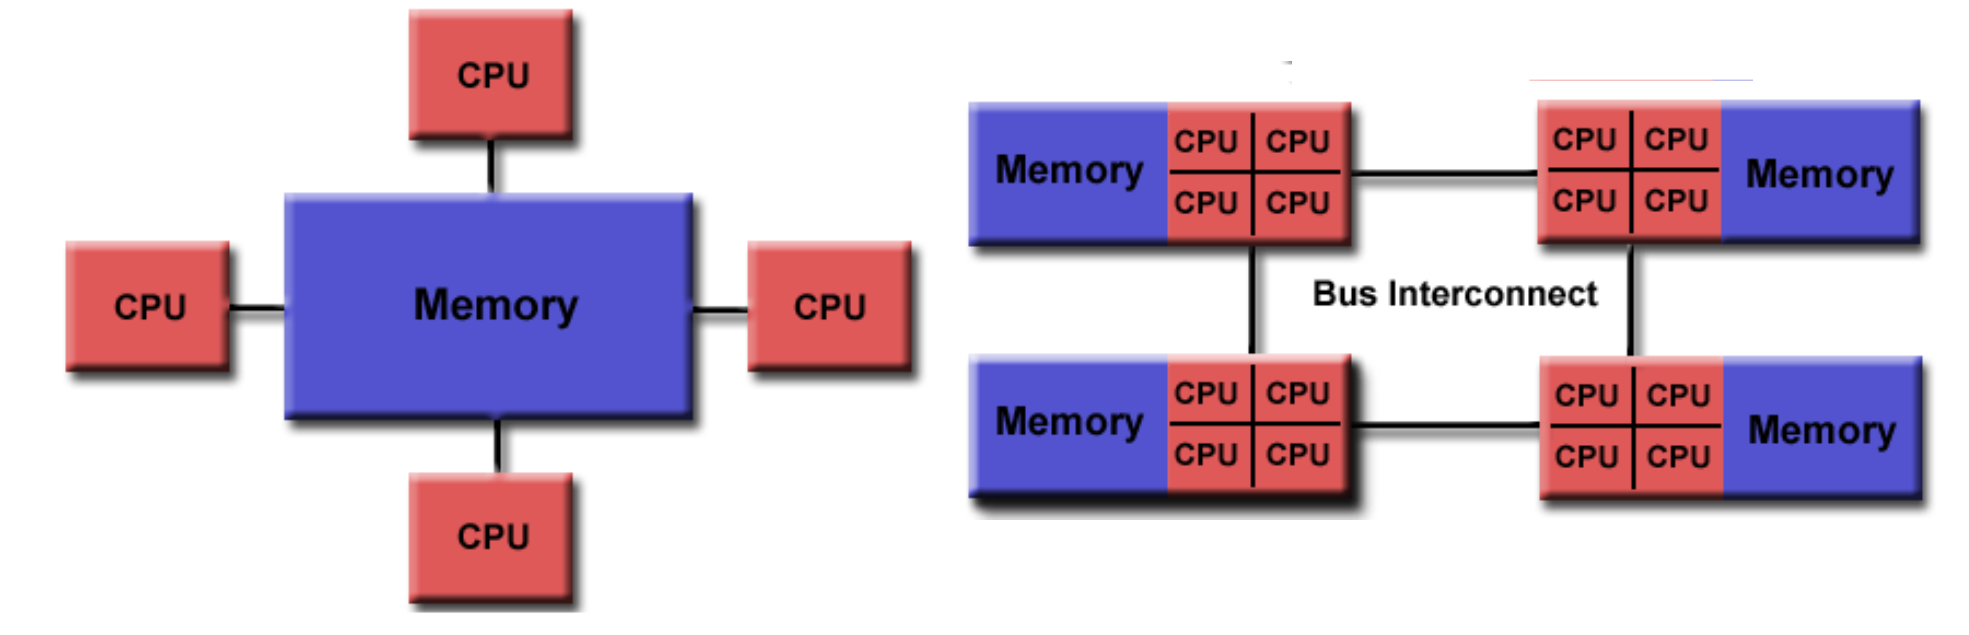
\includegraphics[width=1\textwidth]{pictures/000.png}         
    \caption{ViDuHinhAnhTheoChieuNgang}         
    \label{pictures:000}         
    \end{figure} 
    
    
    
OpenMP sử dụng mô hình fork-join để thực thi song song:
 
\begin{figure}[h]         
    \centering
    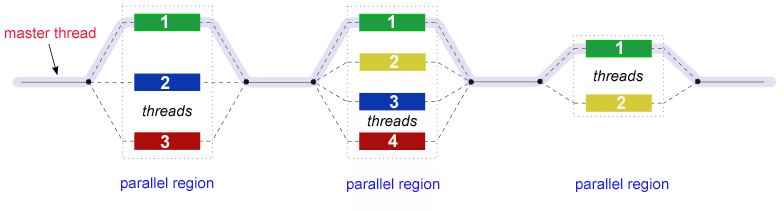
\includegraphics[width=1\textwidth]{pictures/Fork-Join-model-WebSite-4.png}         
    \caption{ViDuHinhAnhTheoChieuNgang}         
    \label{pictures:0001}         
    \end{figure} 



Tất cả các chương trình OpenMP đều bắt đầu dưới dạng một tiến trình duy nhất: luồng chính . Luồng chính thực thi tuần tự cho đến khi gặp cấu trúc vùng song song đầu tiên.


 
\textbf{FORK:}   luồng chính sau đó tạo ra một nhóm các luồng song song .

Sau đó, các câu lệnh trong chương trình được bao quanh bởi cấu trúc vùng song song sẽ được thực thi song song giữa các luồng nhóm khác nhau.

\textbf{JOIN:}         Khi các luồng của nhóm hoàn thành các câu lệnh trong cấu trúc vùng song song, chúng sẽ đồng bộ hóa và chấm dứt, chỉ để lại luồng chính.

 
 
 
 
\newpage
\subsection{Công thức tính hiệu suất}


Công thức tính hiệu suất trong bài báo cáo: 
 

\[\text{{Hiệu suất}} = \frac{{\text{{Thời gian tuần tự}}}}{{\text{{Thời gian song song}} \times \text{{Số luồng}}}}\]
 
 
\subsection{Thông tin về máy tính và phần mềm}


\begin{table}[h]
    \centering
    \begin{tabular}{|l|l|}
        \hline
        \textbf{Thông Tin CPU} & Intel(R) Core(TM) i5-9300H CPU @ 2.40GHz \\
        \hline
        \textbf{Thông Tin RAM} & 16.0 GB \\
        \hline
        \textbf{Hệ Điều Hành} & Windows 11 \\
        \hline
        \textbf{Ngôn Ngữ Lập Trình} & C, C++ \\
        \hline
        \textbf{Trình Biên Dịch} & g++ \\
        \hline
    \end{tabular}
    \caption{Thông Tin Hệ Thống}
    \label{table:system-info}
\end{table}
% \newpage
\section{Giới thiệu chung}
\subsection{Giới thiệu chung về OpenMP}

OpenMP
Fork-Join
Đa luồng là gì
Share memory
% Lập trình đa luồng
\subsection{Công thức tính hiệu suất}




\subsection{Thông tin về máy tính và phần mềm}




 
 
 
\newpage
\section{Thực hành chung}
\subsection{Yêu cầu}
% INPUT
% OUTPUT



\begin{block}{Yêu cầu}  
Thực hiện phép nhân ma trận với vector.

\textbf{INPUT:}  
\begin{itemize}
\item Ma trận  có \(m\) hàng và \(n\) cột. 
\item Vector   có \(n\) phần tử.  
\end{itemize}

\textbf{OUTPUT:}  
\begin{itemize}
\item Vector  kết quả của phép nhân ma trận  với vector.
\end{itemize}
\end{block} 

\subsection{Cơ sở toán học}
Phép nhân ma trận với vector là một phép toán phổ biến trong đại số tuyến tính.

Công thức tính toán như sau:
\[ \mathbf{w} = A \cdot \mathbf{v} \]

Trong đó:
\begin{itemize}
 \item Với \( A \) là ma trận có kích thước \( m \times n \).
 \item Với \( \mathbf{v} \) là vector có kích thước \( n \times 1 \).
 \item Với \( \mathbf{w} \) là vector kết quả có kích thước \( m \times 1 \).
\end{itemize}

Để tính giá trị của \( \mathbf{w} \), thực hiện các phép nhân và cộng tương ứng:
\[ \mathbf{w}_i = \sum_{j=1}^{n} A_{ij} \cdot v_j \]

Trong đó:
\begin{itemize}
 \item Với \( A_{ij} \) là phần tử ở hàng \( i \), cột \( j \) của ma trận \( A \).
 \item Với \( v_j \) là phần tử thứ \( j \) của vector \( \mathbf{v} \).
 \item Với \( \mathbf{w}_i \) là phần tử thứ \( i \) của vector kết quả \( \mathbf{w} \).
\end{itemize}

\textbf{Ví dụ:}
Cho ma trận \( A \) và vector \( \mathbf{v} \) sau:

\[ A = \begin{bmatrix} 1 & 2 & 3 \\ 4 & 5 & 6 \end{bmatrix}, \quad \mathbf{v} = \begin{bmatrix} 2 \\ 1 \\ 3 \end{bmatrix} \]

Phép nhân ma trận \( A \) với vector \( \mathbf{v} \) sẽ tạo ra vector \( \mathbf{w} \) như sau:

\[ \mathbf{w} = A \cdot \mathbf{v} \]

Công thức tính toán:

\[ \begin{bmatrix} w_1 \\ w_2 \end{bmatrix} = \begin{bmatrix} 1 & 2 & 3 \\ 4 & 5 & 6 \end{bmatrix} \cdot \begin{bmatrix} 2 \\ 1 \\ 3 \end{bmatrix} \]

Thực hiện phép nhân và cộng:

\[ w_1 = 1 \cdot 2 + 2 \cdot 1 + 3 \cdot 3 = 13 \]

\[ w_2 = 4 \cdot 2 + 5 \cdot 1 + 6 \cdot 3 = 31 \]

Do đó, vector kết quả \( \mathbf{w} \) là:

\[ \mathbf{w} = \begin{bmatrix} 13 \\ 31 \end{bmatrix} \]

\subsection{Mã nguồn phép nhân ma trận với vector}

\subsubsection{Mã nguồn lập trình tuần tự phép nhân ma trận với vector}
\begin{listing}[H]
 \centering
 \inputminted{cpp}{sources/MaNguon1TT.cpp}
 \caption{Mã nguồn lập trình tuần tự phép nhân ma trận với vector}
 \label{code:MaNguon1TT}
\end{listing}

\subsubsection{Mã nguồn lập trình song song phép nhân ma trận với vector}
\begin{listing}[H]
 \centering
 \inputminted{cpp}{sources/MaNguon1SS.cpp}
 \caption{Mã nguồn lập trình song song phép nhân ma trận với vector}
 \label{code:MaNguon1SS}
\end{listing} 
\newpage
\subsection{Kết quả:}
\subsubsection{Bảng kết quả phép nhân ma trận với vector}




 
\begin{table}[h] %!nghia
 \centering
 \begin{tabular}{|c|c|c|c|}
 
 \hline
 \multicolumn{3}{|c|}{\textbf{BẢNG KẾT QUẢ}} \\ 
 \hline
 \textbf{Kích thước} & \textbf{Thời gian lập trình tuần tự} & \textbf{Thời gian lập trình song song} \\ \hline
 11111111111111111 & 11111111111111111 & 11111111111111111 \\ \hline
 11111111111111111 & 11111111111111111 & 11111111111111111 \\ \hline
 11111111111111111 & 11111111111111111 & 11111111111111111 \\ \hline
 \end{tabular}

 \caption{ViDuBangThuong} %!nghia
 \label{table:nghia1} %!nghia
 \end{table} 
 
 
 
\subsubsection{Biểu đồ phép nhân ma trận với vector}

 
\begin{figure}[h] %!nghia
 \centering
 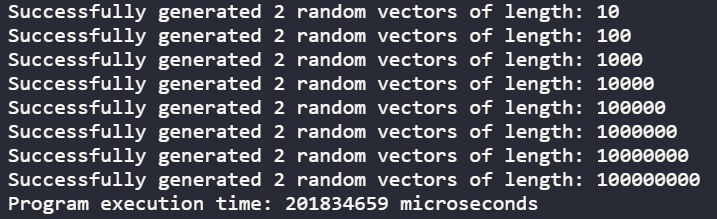
\includegraphics[width=1\textwidth]{pictures/image.png} %!nghia
 \caption{ViDuHinhAnhTheoChieuNgang} %!nghia
 \label{pictures:nghia12} %!nghia
 \end{figure} 
 

\subsection{Nhận xét}
\lipsum[1]



\newpage
\section{Thực hành nhóm}
\subsection{Yêu cầu}
Thực hiện chương trình tính tích vô hướng của 2 vector.
\subsection{Cơ sở toán học}
Tích vô hướng của 2 vector là một phép toán đại số và cho kết quả là một số vô hướng, được tính bằng cách lấy tổng của tích từng cặp phần tử tương ứng:

\[ \mathbf{u} \cdot \mathbf{v} = \sum_{i=1}^{n} u_i \cdot v_i \]

Trong đó:


\begin{itemize}
 \item Với \( \mathbf{u} \) và \( \mathbf{v} \) là hai vector có cùng số chiều \( n \).
 \item Với \( u_i \) và \( v_i \) là phần tử thứ \( i \) của \( \mathbf{u} \) và \( \mathbf{v} \) tương ứng.
\end{itemize}

\textbf{Ví dụ:}

Cho 2 vector \( \mathbf{u} = \langle 1, 2, 3 \rangle \) và \( \mathbf{v} = \langle 4, 5, 6 \rangle \), thì tích vô hướng của \( \mathbf{u} \) và \( \mathbf{v} \) là:

\[ \mathbf{u} \cdot \mathbf{v} = 1 \cdot 4 + 2 \cdot 5 + 3 \cdot 6 = 42\]






\subsection{Mã nguồn tính tích vô hướng của 2 vector}

\subsubsection{Mã nguồn tạo vector ngẫu nhiên}
\begin{listing}[H]
 \centering
 \inputminted{cpp}{sources/MaNguon2NN.cpp}
 \caption{Mã nguồn tạo vector ngẫu nhiên}
 \label{code:MaNguon2NN}
\end{listing}



\subsubsection{Mã nguồn lập trình tuần tự tính tích vô hướng của 2 vector}
\begin{listing}[H]
 \centering
 \inputminted{cpp}{sources/MaNguon2TT.cpp}
 \caption{Mã nguồn lập trình tuần tự tính tích vô hướng của 2 vector}
 \label{code:MaNguon2TT}
\end{listing}




\subsubsection{Mã nguồn lập trình song song tính tích vô hướng của 2 vector}
\begin{listing}[H]
 \centering
 \inputminted{cpp}{sources/MaNguon2SS.cpp}
 \caption{Mã nguồn lập trình song song tính tích vô hướng của 2 vector}
 \label{code:MaNguon2SS}
\end{listing}

Trong mã nguồn sử dụng \texttt{\#pragma omp parallel for reduction(+ : result)} là một chỉ thị được sử dụng trong OpenMP với ý nghĩa:

\begin{enumerate}
 \item \texttt{\#pragma omp}: thông báo cho trình biên dịch hiểu rằng phần mã nguồn sau đó sẽ được thực hiện theo kiểu lập trình đa luồng của OpenMP.

 \item \texttt{parallel for}: thông báo cho trình biên dịch sử dụng đa luồng cho các lần lặp của vòng lặp \texttt{for} tiếp theo.

 \item \texttt{reduction(+ : result)}: sử dụng để chỉ định một toán tử cụ thể. Khi một toán tử được chỉ định, mỗi luồng duy trì một bản sao riêng tư của biến và cuối vùng song song, các kết quả được kết hợp bằng cách sử dụng toán tử đã được chỉ định. Trong mã nguồn này, là phép cộng (\texttt{+}) trên biến \texttt{result}.
\end{enumerate}

Trong ví dụ này, vòng lặp được lập trình đa luồng, và mỗi luồng đóng góp vào tổng của \texttt{result}. Cuối cùng, các kết quả cá nhân của luồng được kết hợp, và tổng cuối cùng được in ra màn hình.








\newpage
\subsection{Kết quả:}
\subsubsection{Bảng kết quả tính tích vô hướng của 2 vector}


 
 \begin{table}[h] %!nghia
 \centering
 \begin{tabular}{|c|c|c|c|}

 \hline
 \multicolumn{3}{|c|}{\textbf{BẢNG KẾT QUẢ}} \\ 
 \hline
 \textbf{Kích thước} & \textbf{Thời gian lập trình tuần tự} & \textbf{Thời gian lập trình song song} \\ \hline
 11111111111111111 & 11111111111111111 & 11111111111111111 \\ \hline
 11111111111111111 & 11111111111111111 & 11111111111111111 \\ \hline
 11111111111111111 & 11111111111111111 & 11111111111111111 \\ \hline
 \end{tabular}

 \caption{ViDuBangThuong} %!nghia
 \label{table:nghia123} %!nghia
 \end{table} 



\subsubsection{Biểu đồ tính tích vô hướng của 2 vector}


 
\begin{figure}[h] %!nghia
\centering
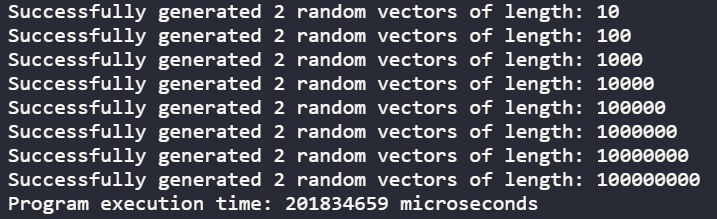
\includegraphics[width=1\textwidth]{pictures/image.png} %!nghia
\caption{ViDuHinhAnhTheoChieuNgang} %!nghia
\label{pictures:nghia1} %!nghia
\end{figure} 






\subsection{Nhận xét}
\lipsum[1]
\newpage
\section*{Kết luận}
\phantomsection \addcontentsline{toc}{section}{Kết luận}

Báo cáo đã trình bày về tính toán song song sử dụng OpenMP cho phép tận dụng xử lý đồng thời với 2 bài toán:

\begin{itemize}
 \item Thực hiện phép nhân ma trận với vector.
 \item Thực hiện chương trình tính tích vô hướng của 2 vector.
\end{itemize}

Việc sử dụng tính toán song song cũng đặt ra một số thách thức như đồng bộ hóa dữ liệu và quản lý tài nguyên.

Thông qua việc thực hiện báo cáo, các thành viên đã được rèn luyện kỹ năng làm việc nhóm và nâng cao khả năng hiểu biết về tính toán song song.

Trong quá trình hoạt động, đôi khi còn khó khăn. Kiến thức và khả năng trình bày của nhóm không tránh khỏi những thiếu sót, rất mong nhận được sự góp ý và bổ sung.

\newpage
\section*{Tài liệu tham khảo}
\phantomsection \addcontentsline{toc}{section}{Tài liệu tham khảo}

\begin{enumerate}[label=(\arabic*)]
 \item \url{https://en.wikipedia.org/wiki/Parallel_computing}
 \item \url{https://en.wikipedia.org/wiki/OpenMP}
 \item \url{https://en.wikipedia.org/wiki/Matrix_multiplication}
 \item \url{https://en.wikipedia.org/wiki/Dot_product}
 \item \url{https://hpc-tutorials.llnl.gov/openmp}
 \item \url{https://www.youtube.com/watch?v=JpU53_G-HAk}
 \item \url{https://hpc.llnl.gov/documentation/tutorials/introduction-parallel-computing-tutorial}
 
\end{enumerate}
%%%%%%%%%%%%%%%%%%%%%%%%%%%%%%%%%%%%%%%%%%%%%%%%%%%%% 
\end{document}

